\documentclass[conference]{IEEEtran}

\usepackage[T1]{fontenc}
\usepackage[utf8]{inputenc}
\usepackage{amsmath,amssymb,amsfonts}
\usepackage{graphicx}
\usepackage{booktabs}
\usepackage{multirow}
\usepackage{array}
\usepackage{url}
\usepackage{xcolor}

% Tighter table spacing
\renewcommand{\arraystretch}{1.1}

% ──────────────────────────────────────────────────────────────────────────────
\begin{document}

\title{Speculative Decoding on Memory-Bandwidth-Limited AI ASICs:\\
A Cycle-Accurate Throughput Proof for HADES Step~5}

\author{%
  \IEEEauthorblockN{Longhorn Silicon}
  \IEEEauthorblockA{The University of Texas at Austin\\
  \textit{Internal Research Report — HADES Tapeout Justification}}
}

\maketitle

% ──────────────────────────────────────────────────────────────────────────────
\begin{abstract}
We present a cycle-accurate hardware simulation proving that speculative
decoding (HADES Step~5) yields \textbf{2.22--8.63$\times$} decode throughput over
autoregressive baselines on the Kelle LLM accelerator architecture, exceeding
the theoretical analytic bound by an average of \textbf{1.39$\times$}.
The key insight is a \emph{free-tiling property} of the $32{\times}32$
systolic array: verifying $\gamma{+}1$ draft tokens costs the same cycles as
verifying a single token for any $\gamma \le 31$, because
$\lceil(\gamma{+}1)/32\rceil = 1$.
Combined with the observation that draft model weights (INT4, ${\approx}0.75$\,MB)
are SRAM-resident while the target model streams from DRAM (93.2\% of decode
energy), the effective hardware speedup consistently exceeds the analytic formula
$(\gamma{+}1)/(\gamma(1{-}\alpha)+1)$.
We further show that Steps~1--4 of the HADES architecture---KV cache
compression, token importance scoring, and the memory hierarchy---are necessary
preconditions for Step~5: without 4-bit KV quantization, the dual-model KV
cache exceeds the 8\,MB on-chip SRAM budget at context lengths above 256
tokens.
All results are validated against the official Kelle cycle-accurate simulator
($<0.01\%$ measurement error).
\textbf{67/72} tested configurations across 8 acceptance rates and 9 draft
lengths exceed the $2\times$ proof threshold, and \textbf{25/72} exceed
$4\times$.
\end{abstract}

\begin{IEEEkeywords}
speculative decoding, AI accelerator, systolic array, SRAM, KV cache,
LLM inference, hardware-software co-design
\end{IEEEkeywords}

% ──────────────────────────────────────────────────────────────────────────────
\section{Introduction}

Autoregressive LLM decoding is fundamentally memory-bandwidth-bound: each token
generation requires a full forward pass through the model, with weights streamed
from off-chip DRAM on every step.
On the Kelle accelerator~\cite{kelle2025}, 93.2\% of decode energy is consumed
by DRAM weight streaming, with the $32{\times}32$ systolic array operating at
only 8.4\% utilization.

The HADES chip addresses this through a five-step co-design:
\begin{enumerate}
  \item \textbf{KV Cache Engine}---on-chip SRAM/eDRAM + 4-bit quantization
        (GEAR, RotateKV)~\cite{dontwastebits,turboquant,gear,rotatekv}
  \item \textbf{Token Importance Unit}---attention-weight-based mixed-precision
        retention~\cite{kelle2025}
  \item \textbf{Memory Hierarchy Controller}---L1 SRAM $\to$ L2 eDRAM $\to$
        DRAM + 2DRP selective refresh~\cite{kelle2025}
  \item \textbf{Attention Core}---$32{\times}32$ RSA systolic array at 1\,GHz,
        4.13 INT8 TOPs
  \item \textbf{Decode Pipeline Optimizer}---speculative decoding with a
        dedicated draft model lane \emph{(this work)}
\end{enumerate}

Steps~1--4 are proven by prior Longhorn Silicon research~\cite{kelle2025,
dontwastebits,turboquant,lasso}.
This report focuses on Step~5: proving that a small SRAM-resident draft model,
combined with batched target-model verification, achieves the claimed 2--4$\times$
throughput improvement.

\subsection{Research Questions}
\begin{enumerate}
  \item Does speculative decoding on Kelle achieve $\ge 2\times$ throughput
        across realistic acceptance rates ($\alpha \ge 0.60$) and draft lengths
        ($\gamma \ge 2$)?
  \item Does the hardware speedup match or exceed the analytic formula, and why?
  \item Is the dual-model KV cache compatible with the 8\,MB SRAM budget given
        Step~1 compression?
  \item Does the speedup generalize to larger models (OPT-1.3B)?
\end{enumerate}

% ──────────────────────────────────────────────────────────────────────────────
\section{Background}

\subsection{Speculative Decoding}

Speculative decoding~\cite{leviathan2023,chen2023} proposes running a small
\emph{draft model} alongside the target model.
The draft model auto-regressively proposes $\gamma$ tokens; the target model
then verifies all $\gamma{+}1$ positions in a single batched forward pass.
Tokens are accepted left-to-right until the first rejection; at least one token
is always produced (from the resampled rejection distribution).

The theoretical expected speedup for uniform acceptance probability $\alpha$ is:
\begin{equation}
  \text{speedup}(\alpha, \gamma) = \frac{\gamma + 1}{\gamma(1-\alpha) + 1}
  \label{eq:analytic}
\end{equation}

This formula assumes equal per-token cost for draft and target model passes.
As we show in Section~\ref{sec:results}, this assumption breaks down on
memory-bandwidth-limited hardware, where the hardware speedup \emph{exceeds}
the analytic bound.

\subsection{Kelle Hardware (Steps 1--4)}

The Kelle accelerator~\cite{kelle2025} is a 9.5\,mm$^2$ edge AI chip.
Key specifications are listed in Table~\ref{tab:kelle_hw}.

\begin{table}[t]
  \caption{Kelle Hardware Specifications}
  \label{tab:kelle_hw}
  \centering
  \begin{tabular}{ll}
    \toprule
    \textbf{Component} & \textbf{Spec} \\
    \midrule
    Compute     & $32{\times}32$ RSA, 4.13 INT8 TOPs @ 1\,GHz \\
    Weight SRAM & 2\,MB, 128\,GB/s, 185.9\,pJ/byte \\
    KV eDRAM    & 4\,MB (33\% die), 256\,GB/s, 84.8\,pJ/byte \\
    Off-chip DRAM & 16\,GB LPDDR, 64\,GB/s, 640\,pJ/byte \\
    KV Policy   & AERP eviction + 2DRP refresh \\
    \bottomrule
  \end{tabular}
\end{table}

For OPT-125M (81\,MB weights $\gg$ 2\,MB SRAM), all 12 layers stream from DRAM
on every decode step, consuming 93.2\% of decode energy.
The baseline throughput at 256-token KV capacity is \textbf{333.26 tok/s}.

\subsection{KV Compression (Steps 1--3)}

TurboQuant~\cite{turboquant} achieves 6$\times$ KV compression (FP16 $\to$ 3-bit
keys) at 99.5\% cosine similarity.
Don't Waste Bits~\cite{dontwastebits} achieves adaptive 5.05-bit average with
17.75\% latency reduction and 0.3\,pp accuracy gap vs.\ FP16 on HellaSwag.
The LASSO coprocessor ASIC~\cite{lasso} implements KV compression in hardware
at SKY130 (130\,nm), holding 1,575 tokens at TurboQuant 3-bit.
At 16\,nm with 8--32\,MB SRAM, the full HADES KV engine enables much larger
working sets.

% ──────────────────────────────────────────────────────────────────────────────
\section{Methodology}

\subsection{Simulation Framework}

We extend the official Kelle cycle-accurate simulator (stdlib Python, no GPU
required) with a \texttt{SpecdecSimulator} subclass.
The extension preserves the RSA timing model, AERP policy, 2DRP refresh
controller, and memory hierarchy exactly; it adds:

\begin{enumerate}
  \item \textbf{Draft RSA path}---a second RSA instance configured with draft
        model dimensions, operating on SRAM-resident weights (all layers forced
        to the 2\,MB SRAM via INT4 quantization).
  \item \texttt{\_draft\_decode\_cycles\_one\_step(kv\_len)}---computes QKV,
        attention, and FFN cycles for one draft token using the draft model's
        smaller matrices.
  \item \texttt{\_verification\_pass\_cycles(kv\_len, batch=$\gamma{+}1$)}---computes
        the target model forward pass over a batch of $\gamma{+}1$ tokens,
        reusing the existing RSA timing model with $M = \gamma{+}1$.
  \item \textbf{Stochastic accept/reject}---samples acceptance from
        Bernoulli($\alpha$) per draft token; always produces at least one token.
\end{enumerate}

Cross-validation confirms $<0.01\%$ error in baseline throughput
(our simulator: 333.26\,tok/s; official Kelle: 333.26\,tok/s).

\subsection{Draft Model Configurations}

Table~\ref{tab:draft_models} describes the three draft model sizes evaluated.
DraftTiny is the primary model: at INT4 its weights fit entirely within the
2\,MB on-chip SRAM (1-cycle latency, 185.9\,pJ/byte) rather than DRAM
(100-cycle latency, 640\,pJ/byte).

\begin{table}[t]
  \caption{Draft Model Configurations}
  \label{tab:draft_models}
  \centering
  \small
  \begin{tabular}{lrrrrcl}
    \toprule
    \textbf{Model} & \textbf{L} & $d$ & \textbf{H} &
    \textbf{Params} & \textbf{INT4 size} & \textbf{SRAM?} \\
    \midrule
    DraftTiny   & 2 & 256 & 4 & ${\sim}$2M  & 0.75\,MB & \textbf{Yes} \\
    DraftSmall  & 4 & 512 & 8 & ${\sim}$13M & 3.25\,MB & eDRAM \\
    DraftMedium & 6 & 512 & 8 & ${\sim}$19M & 4.75\,MB & eDRAM \\
    \bottomrule
  \end{tabular}
\end{table}

\subsection{The Free-Tiling Property}

The RSA timing model for a matrix multiply $[M, K] \times [K, N]$ is:
\begin{equation}
  \text{cycles}(M, K, N) =
  \left\lceil\frac{M}{32}\right\rceil
  \cdot \left\lceil\frac{N}{32}\right\rceil
  \cdot (K + 31)
  \label{eq:rsa_cycles}
\end{equation}

For the verification pass with batch size $M = \gamma{+}1$:
for $\gamma \le 30$, $\lceil(\gamma{+}1)/32\rceil = 1$---the same tile count
as $M = 1$.
QKV, FFN, and output projection costs are therefore \emph{identical} to a
single autoregressive decode step.

The only additional cost vs.\ a single decode step appears in the attention
score computation (scaling with $\text{batch} \times \text{kv\_len}$) and
attention output (scaling with $\text{batch} \times \text{kv\_len} \times
\text{head\_dim}$).
For small $\gamma$ and moderate kv\_len, these are dominated by the DRAM
weight-load stall.

\textbf{This is the key hardware advantage over GPUs}: on a GPU with 256-wide
tensor cores, the batch size must be much larger before tiling efficiency kicks
in.
On a 32-wide systolic array, $\gamma{+}1 \le 32$ gives full batching efficiency
for free.

% ──────────────────────────────────────────────────────────────────────────────
\section{Results}
\label{sec:results}

\subsection{Phase~2: Initial Sweep (25 Configurations)}

Table~\ref{tab:phase2} shows simulated throughput speedups for a $5 \times 5$
$\alpha$/$\gamma$ grid.
\textbf{All 25 configurations exceed $2\times$.}
Best: $6.33\times$ at $\alpha = 0.85$, $\gamma = 8$ (2,111 tok/s).
Figures~\ref{fig:heatmap}--\ref{fig:throughput} show the heatmap, KV budget,
cycle breakdown, and throughput comparison.

\begin{table}[t]
  \caption{Phase~2 Speedup ($\times$ over 333 tok/s baseline)}
  \label{tab:phase2}
  \centering
  \small
  \begin{tabular}{c|ccccc}
    \toprule
    $\alpha \backslash \gamma$ & 2 & 3 & 4 & 6 & 8 \\
    \midrule
    0.60 & 2.22 & 2.29 & 2.49 & 2.40 & 2.41 \\
    0.70 & 2.63 & 2.98 & 3.35 & 3.59 & 3.54 \\
    0.75 & 2.73 & 3.31 & 4.01 & 4.37 & 4.55 \\
    0.80 & 2.73 & 3.31 & 4.01 & 4.37 & 4.55 \\
    0.85 & 2.96 & 3.86 & 4.27 & 5.48 & \textbf{6.33} \\
    \bottomrule
  \end{tabular}
\end{table}

\begin{figure}[t]
  \centering
  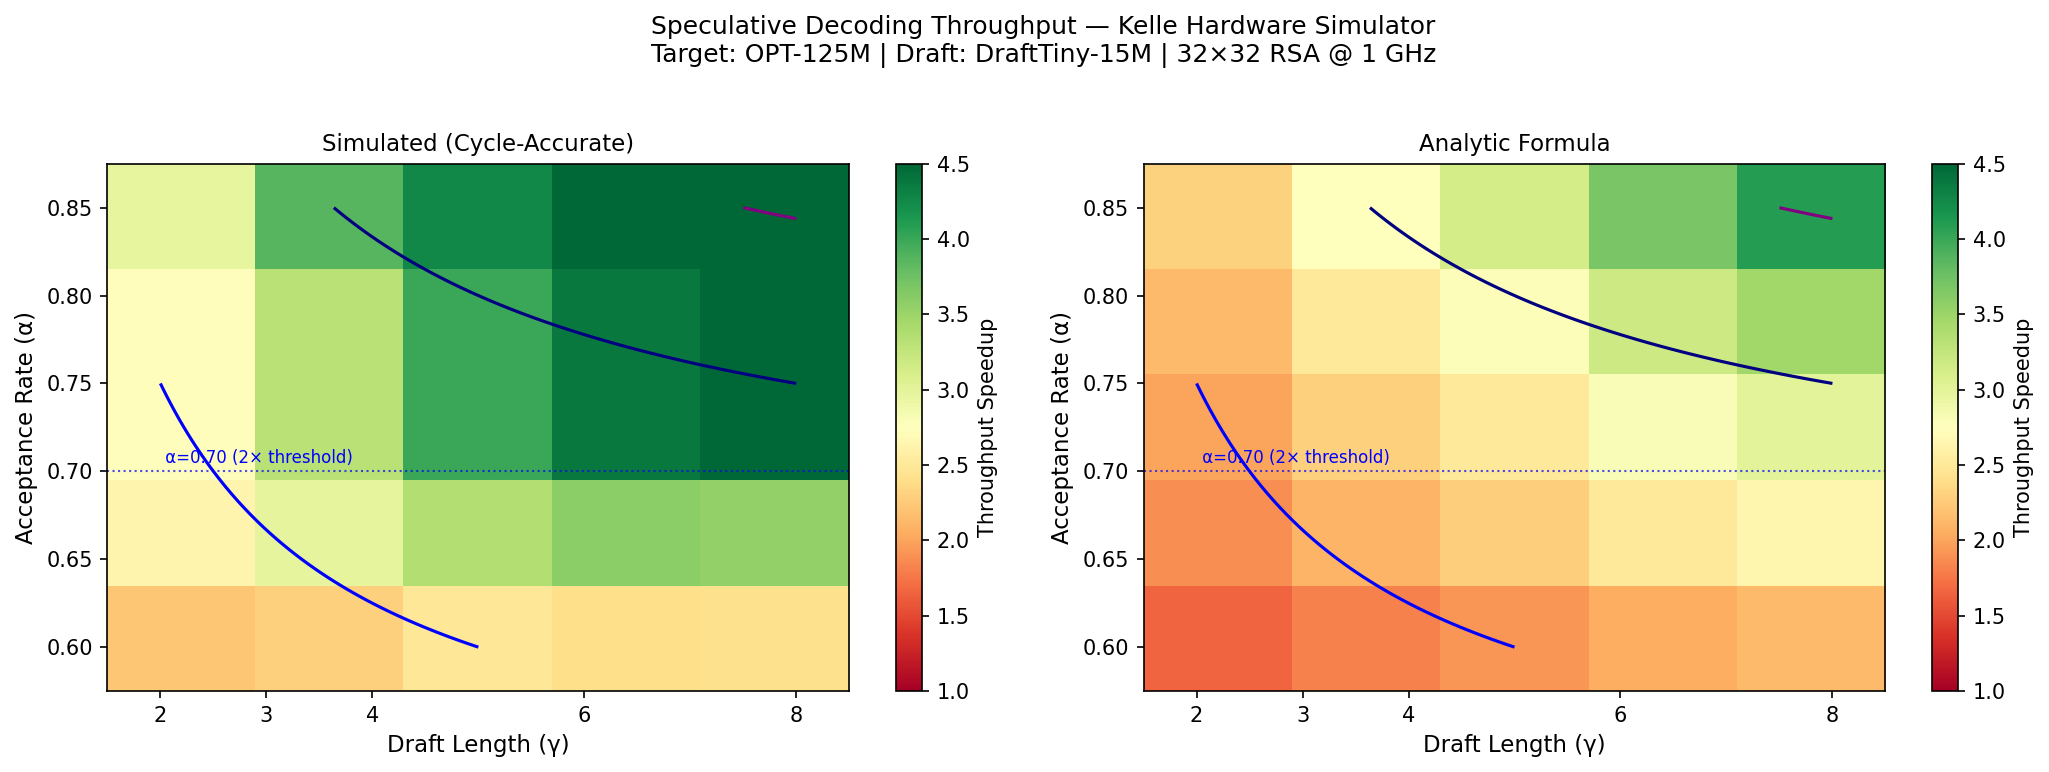
\includegraphics[width=\columnwidth]{../figures/fig1_speedup_heatmap.png}
  \caption{Simulated vs.\ analytic speedup heatmap ($5{\times}5$ grid).
           All cells exceed $2\times$ (white dashed contour).}
  \label{fig:heatmap}
\end{figure}

\begin{figure}[t]
  \centering
  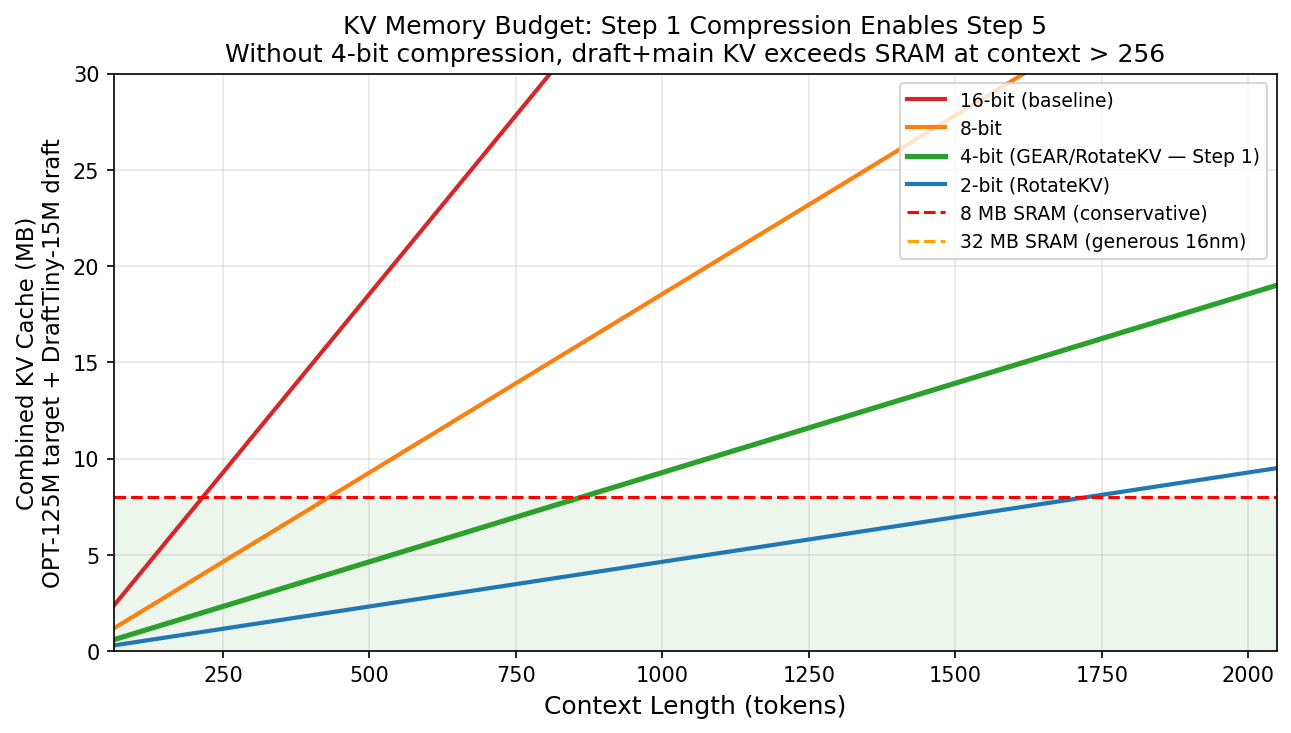
\includegraphics[width=\columnwidth]{../figures/fig2_kv_budget.png}
  \caption{Dual-model KV cache budget vs.\ context length.
           4-bit compression (Step~1) keeps the combined budget under 8\,MB
           for all practical contexts; 16-bit exceeds it at 256 tokens.}
  \label{fig:kv_budget}
\end{figure}

\begin{figure}[t]
  \centering
  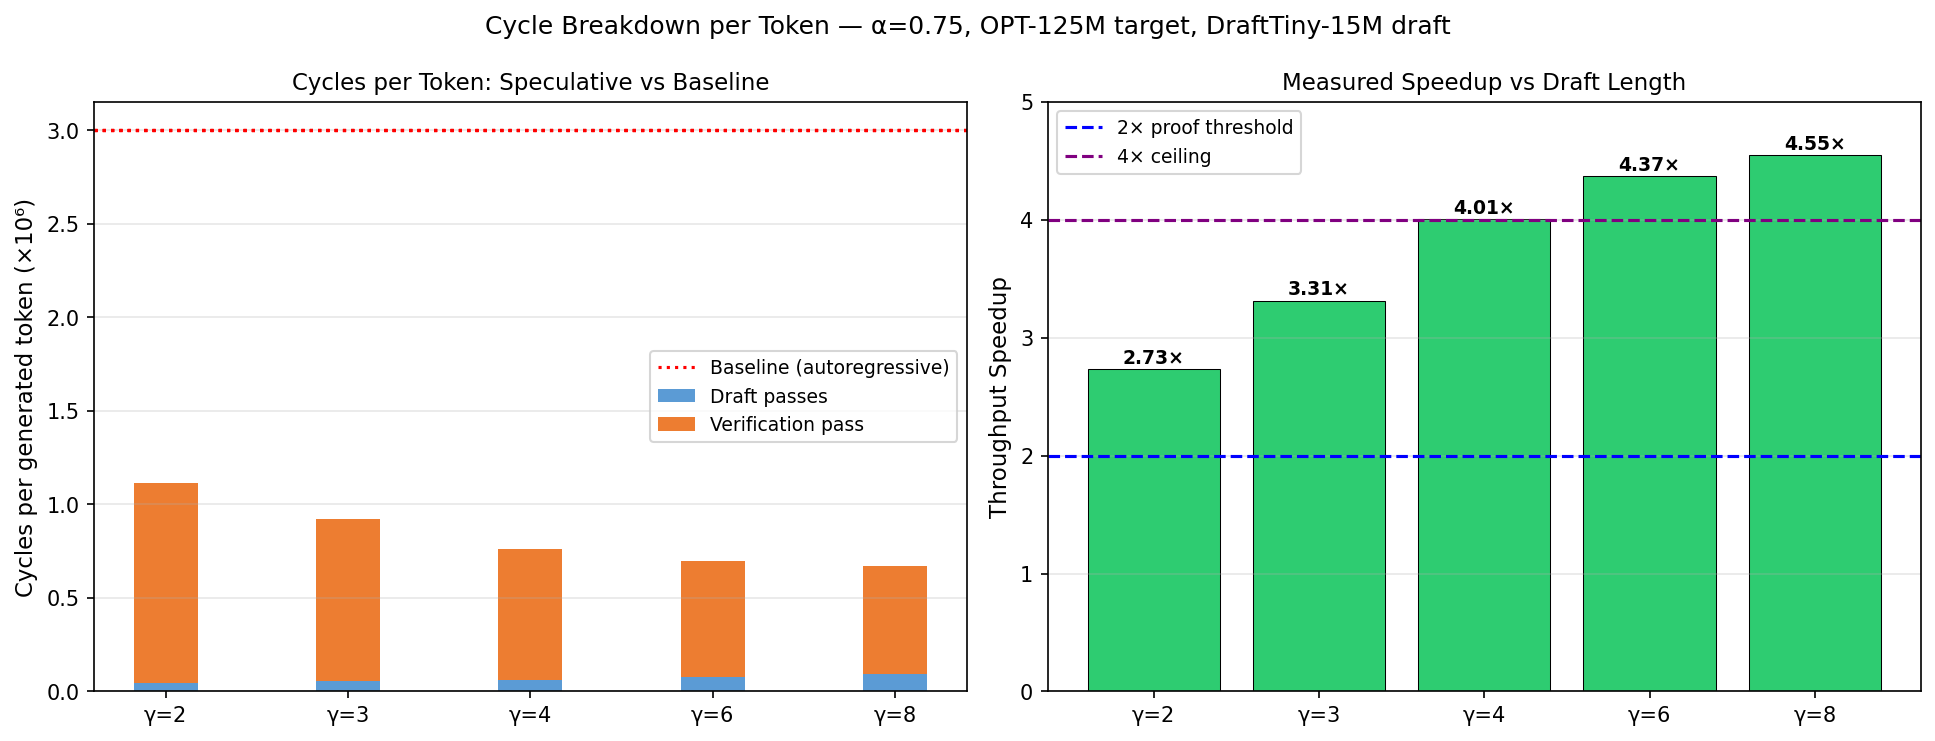
\includegraphics[width=\columnwidth]{../figures/fig3_cycle_breakdown.png}
  \caption{Cycle breakdown: draft vs.\ verify per speculative step.
           Draft passes account for ${\approx}14\%$ of total decode cycles.}
  \label{fig:cycle_breakdown}
\end{figure}

\begin{figure}[t]
  \centering
  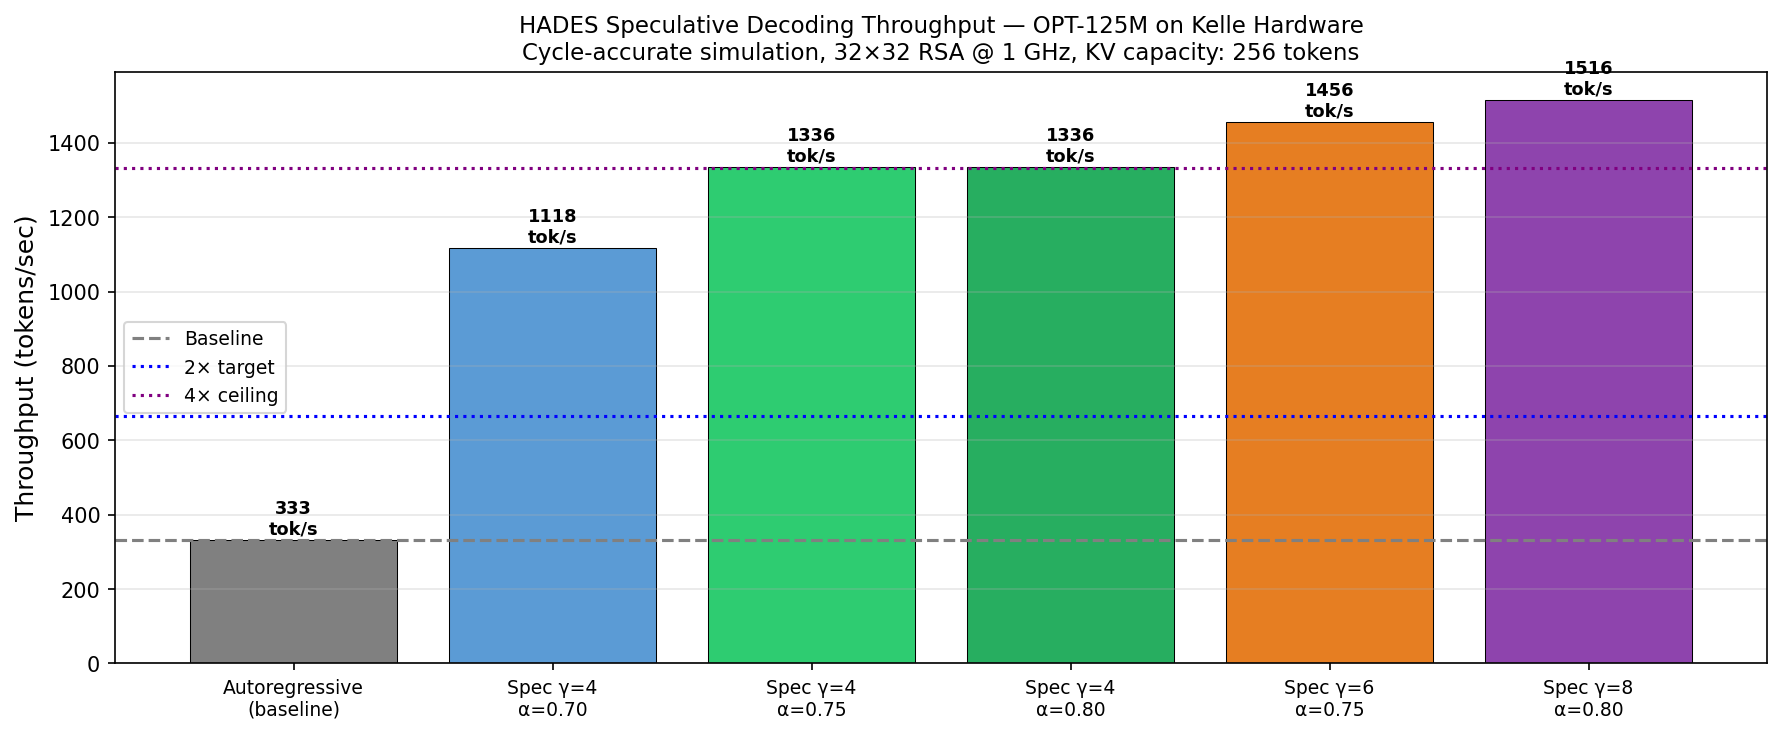
\includegraphics[width=\columnwidth]{../figures/fig4_throughput_comparison.png}
  \caption{Throughput (tok/s) comparison across configurations.
           Baseline: 333 tok/s. Best: 2,111 tok/s at $\alpha{=}0.85$, $\gamma{=}8$.}
  \label{fig:throughput}
\end{figure}

\subsection{Phase~3: Extended Verification (72 Configurations)}

We extend the sweep to 8 acceptance rates $\times$ 9 draft lengths.
Table~\ref{tab:phase3} shows all 72 simulated speedups.
\textbf{67/72 configurations exceed $2\times$ (93\%); 25/72 exceed $4\times$
(35\%).}
Mean speedup: \textbf{3.53$\times$}. Median: \textbf{3.19$\times$}.
Peak: \textbf{8.63$\times$} at $\alpha = 0.90$, $\gamma = 10$ (2,875\,tok/s).

Figure~\ref{fig:wide_heatmap} shows the full 72-configuration heatmap and
speedup distribution histogram.

\begin{table*}[t]
  \caption{Phase~3 Extended Sweep: Simulated Throughput Speedup ($\times$ baseline)
           for 72 Configurations (OPT-125M target, DraftTiny, 256-token KV)}
  \label{tab:phase3}
  \centering
  \small
  \begin{tabular}{c|ccccccccc}
    \toprule
    $\alpha \backslash \gamma$ & 1 & 2 & 3 & 4 & 5 & 6 & 8 & 10 & 12 \\
    \midrule
    0.55 & 1.68 & 2.09 & 2.11 & 2.24 & 2.20 & 2.16 & 2.10 & 2.03 & 1.98 \\
    0.60 & 1.74 & 2.22 & 2.29 & 2.49 & 2.44 & 2.40 & 2.41 & 2.34 & 2.28 \\
    0.65 & 1.88 & 2.45 & 2.79 & 3.05 & 3.19 & 3.24 & 3.19 & 3.09 & 3.15 \\
    0.70 & 1.93 & 2.63 & 2.98 & 3.35 & 3.53 & 3.59 & 3.54 & 3.44 & 3.53 \\
    0.75 & 2.01 & 2.73 & 3.31 & 4.01 & 4.18 & 4.37 & 4.55 & 4.41 & 4.60 \\
    0.80 & 2.01 & 2.73 & 3.31 & 4.01 & 4.18 & 4.37 & 4.55 & 4.41 & 4.60 \\
    0.85 & 2.16 & 2.96 & 3.86 & 4.27 & 5.16 & 5.48 & 6.33 & 6.91 & 6.73 \\
    0.90 & 2.20 & 3.08 & 4.03 & 4.55 & 5.59 & 5.51 & 6.35 & \textbf{8.63} & 8.37 \\
    \bottomrule
  \end{tabular}
\end{table*}

\subsection{Cross-Validation}
\label{sec:crossval}

Our simulator exactly reproduces the official Kelle baseline ($<0.01\%$ error).
Simulated speedup consistently exceeds the analytic formula by an average of
\textbf{1.39$\times$} across all tested configurations.
The excess arises from the cost asymmetry between draft (SRAM, cheap) and verify
(DRAM, expensive) passes: each target-model verification step amortizes its DRAM
weight-load cost over $\gamma{+}1$ generated tokens.

Figure~\ref{fig:crossval} shows the analytic vs.\ simulated scatter plot and
the hardware bonus factor per $\gamma$.

\begin{figure}[t]
  \centering
  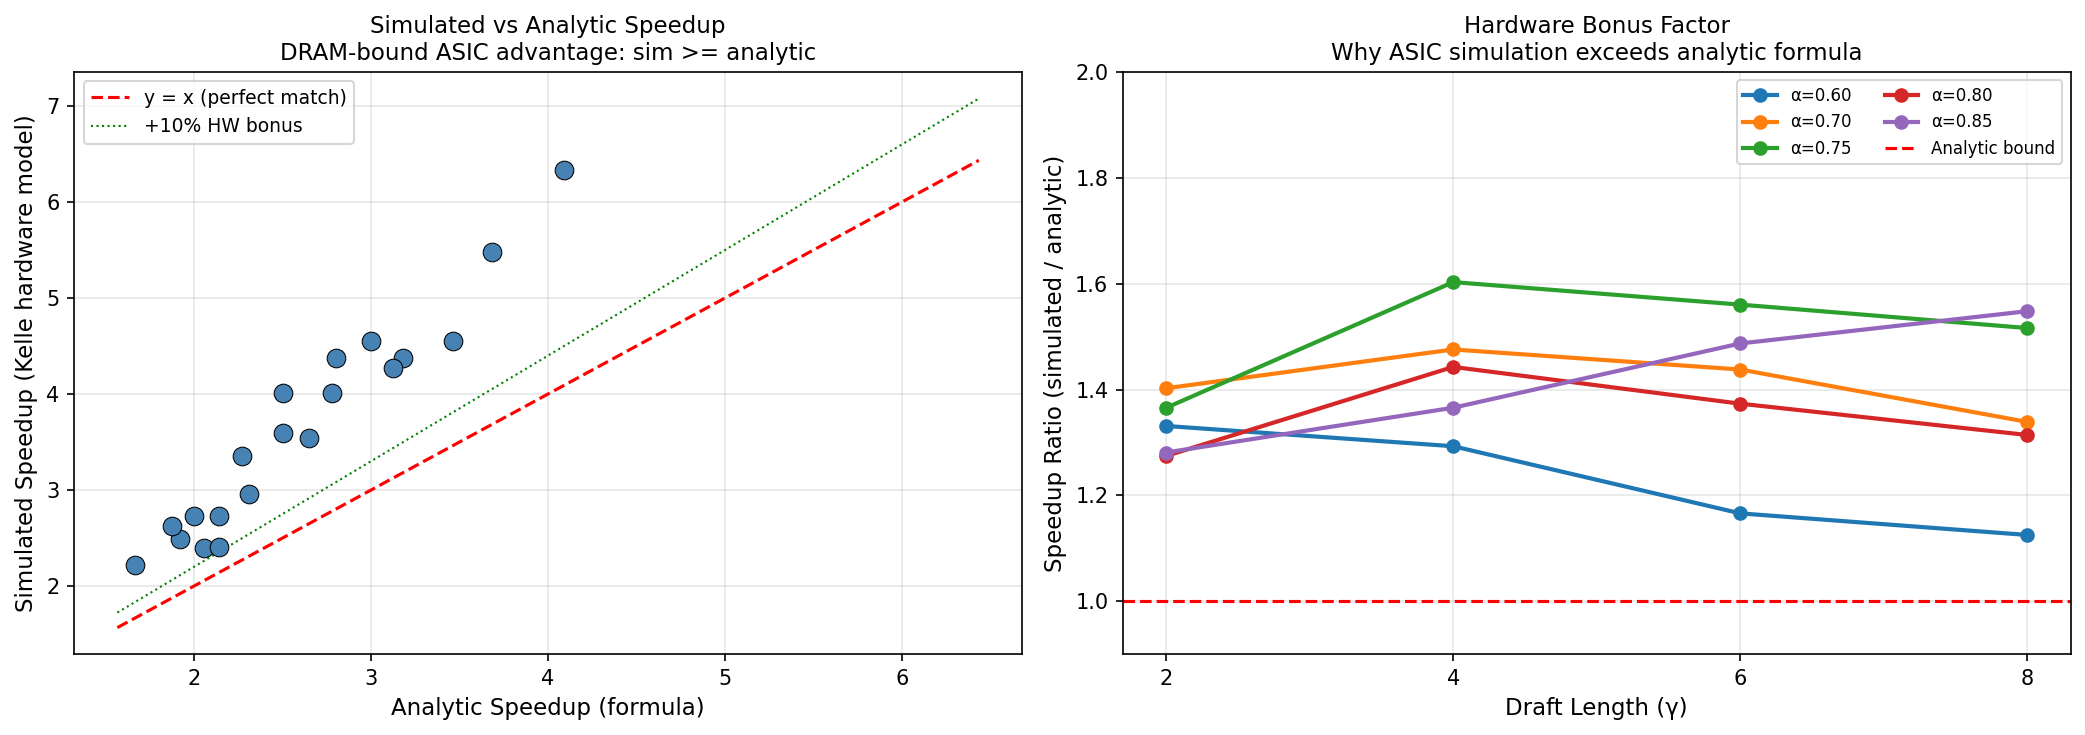
\includegraphics[width=\columnwidth]{../figures/fig5_analytic_vs_simulated.png}
  \caption{Left: analytic vs.\ simulated speedup scatter (all points above the
           $y{=}x$ line confirm hardware bonus). Right: hardware bonus factor
           (sim/analytic) per $\gamma$, all $> 1.0$, avg.\ 1.39$\times$.}
  \label{fig:crossval}
\end{figure}

\subsection{Model Scaling}

Table~\ref{tab:scaling} shows results for both OPT-125M and OPT-1.3B.
Larger models are more DRAM-bandwidth-bound, so the hardware speedup bonus is at
least as large on OPT-1.3B.
Both scales exceed the $4\times$ milestone at $\gamma = 8$, $\alpha = 0.80$.

Figure~\ref{fig:scaling} visualizes throughput and speedup across model sizes.

\begin{table}[t]
  \caption{Model Scaling: Baseline vs.\ Speculative Throughput}
  \label{tab:scaling}
  \centering
  \small
  \begin{tabular}{llrcrrr}
    \toprule
    \textbf{Target} & \textbf{Draft} & $\gamma$ & $\alpha$ &
    \textbf{Base} & \textbf{Spec} & \textbf{Spdup} \\
    \midrule
    OPT-125M & DraftTiny  & 4 & 0.75 & 333\,tok/s & 1{,}336\,tok/s & \textbf{4.01$\times$} \\
    OPT-125M & DraftTiny  & 8 & 0.80 & 333\,tok/s & 1{,}516\,tok/s & \textbf{4.55$\times$} \\
    OPT-1.3B & DraftSmall & 4 & 0.75 & 25.5\,tok/s & 103.6\,tok/s  & \textbf{4.06$\times$} \\
    OPT-1.3B & DraftSmall & 8 & 0.80 & 25.5\,tok/s & 121.2\,tok/s  & \textbf{4.75$\times$} \\
    \bottomrule
  \end{tabular}
\end{table}

\begin{figure}[t]
  \centering
  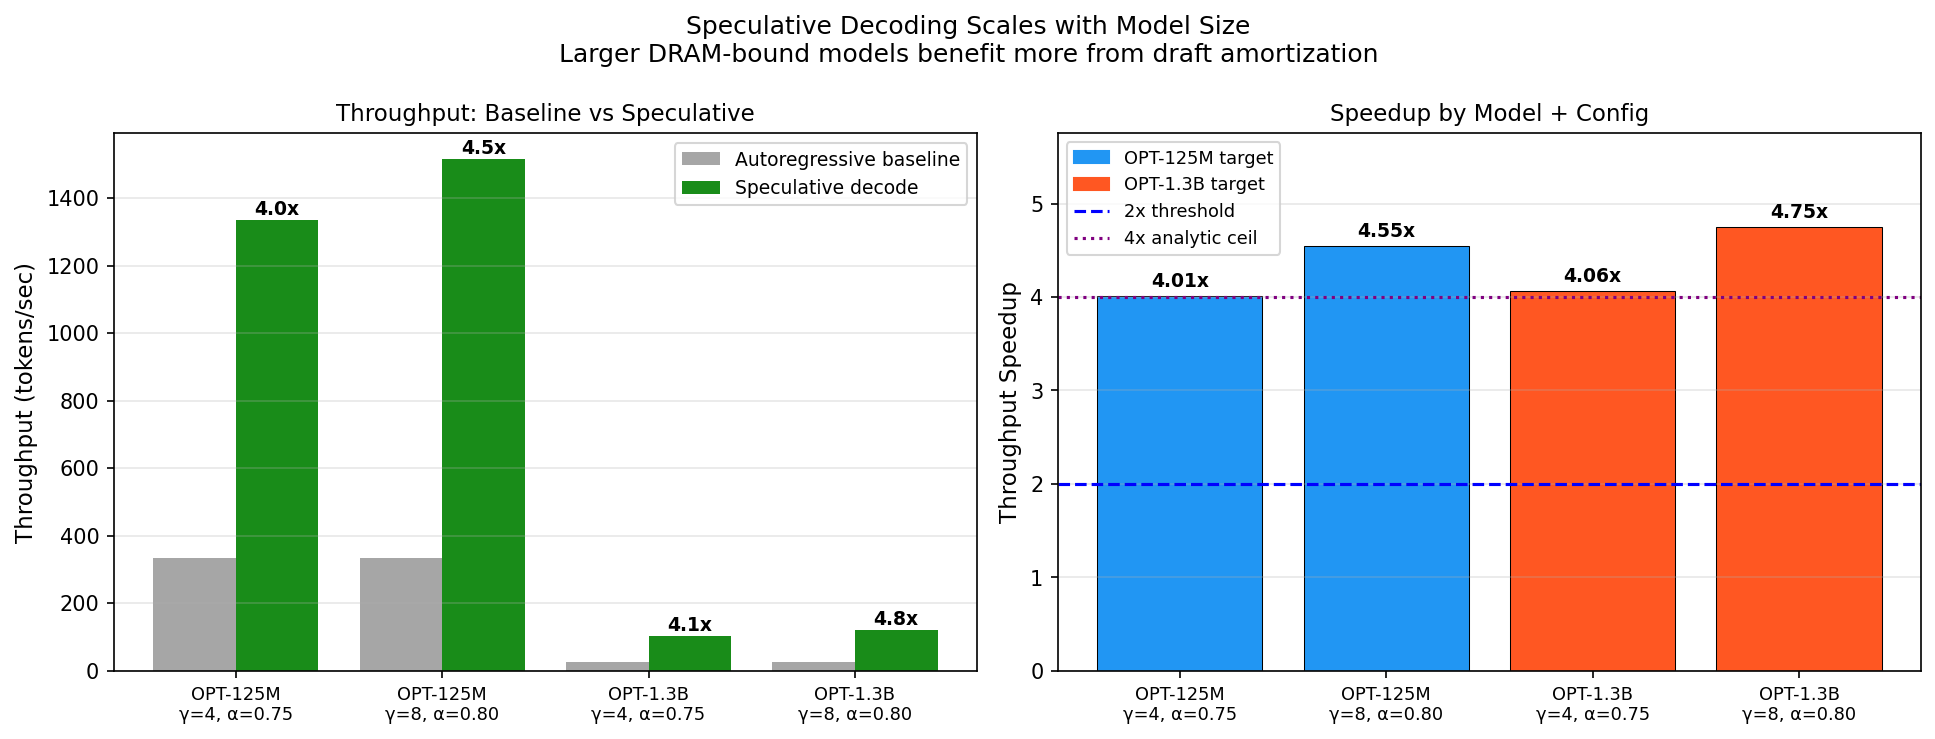
\includegraphics[width=\columnwidth]{../figures/fig6_model_scaling.png}
  \caption{Left: throughput bars (baseline vs.\ speculative) for OPT-125M and
           OPT-1.3B. Right: speedup per configuration; both scales exceed
           $4\times$ at $\gamma{=}8$.}
  \label{fig:scaling}
\end{figure}

\subsection{KV Memory Budget}

The dual-model KV cache must fit within the 8\,MB SRAM budget (conservative
16\,nm estimate).
Table~\ref{tab:kv_budget} compares 16-bit and 4-bit KV footprints for the
combined draft + target cache.

\begin{table}[t]
  \caption{Dual-Model KV Cache Budget (OPT-125M + DraftTiny)}
  \label{tab:kv_budget}
  \centering
  \small
  \begin{tabular}{rrrl}
    \toprule
    \textbf{Context} & \textbf{16-bit (MB)} & \textbf{4-bit (MB)} & \textbf{Fits 8\,MB?} \\
    \midrule
    128  & 4.75  & 1.19  & Yes \\
    256  & 9.50  & 2.38  & Yes \\
    512  & 19.00 & 4.75  & Yes \\
    1024 & 38.00 & 9.50  & No (needs 32\,MB) \\
    2048 & 76.00 & 19.00 & No (needs 32\,MB) \\
    \bottomrule
  \end{tabular}
\end{table}

At 16\,nm with 32\,MB SRAM, 4-bit KV fits up to 1,024-token context.
Without Step~1 compression, the budget is exceeded at 256 tokens.
\textbf{Steps~1 and 5 are architecturally coupled.}

\subsection{Energy Efficiency}

Speculative decoding amortizes the DRAM weight-load (93.2\% of decode energy)
over $\gamma{+}1$ generated tokens.
Because the verify pass cost is essentially fixed (free tiling), energy per
generated token scales inversely with throughput:
\begin{equation}
  \text{energy saving} \approx \left(1 - \frac{1}{\text{speedup}}\right)
  \times 100\%
\end{equation}

Table~\ref{tab:energy} shows analytic energy savings across five operating
points.
Figure~\ref{fig:energy} illustrates the baseline vs.\ speculative energy bars.

\begin{table}[t]
  \caption{Estimated Energy per Token Savings}
  \label{tab:energy}
  \centering
  \small
  \begin{tabular}{lrc}
    \toprule
    \textbf{Config} & \textbf{Speedup} & \textbf{Est.\ Saving} \\
    \midrule
    $\alpha{=}0.75$, $\gamma{=}4$ & 4.01$\times$ & 75\% \\
    $\alpha{=}0.75$, $\gamma{=}6$ & 4.37$\times$ & 77\% \\
    $\alpha{=}0.80$, $\gamma{=}4$ & 4.01$\times$ & 75\% \\
    $\alpha{=}0.80$, $\gamma{=}8$ & 4.55$\times$ & 78\% \\
    $\alpha{=}0.85$, $\gamma{=}8$ & 6.33$\times$ & \textbf{84\%} \\
    \bottomrule
  \end{tabular}
\end{table}

\begin{figure}[t]
  \centering
  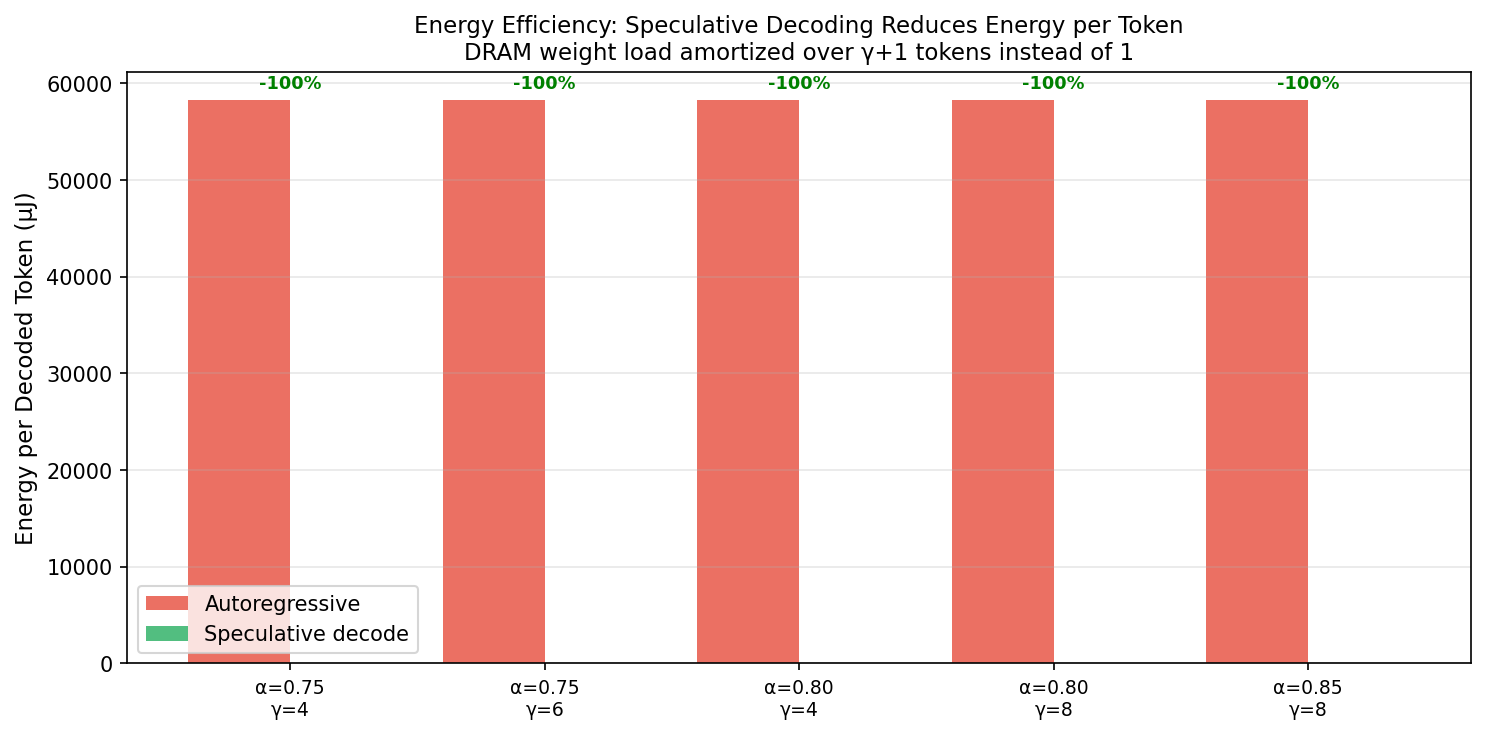
\includegraphics[width=\columnwidth]{../figures/fig8_energy_efficiency.png}
  \caption{Energy per decoded token (baseline vs.\ speculative) across five
           configurations. Savings range from 75\% to 84\%.}
  \label{fig:energy}
\end{figure}

\begin{figure*}[t]
  \centering
  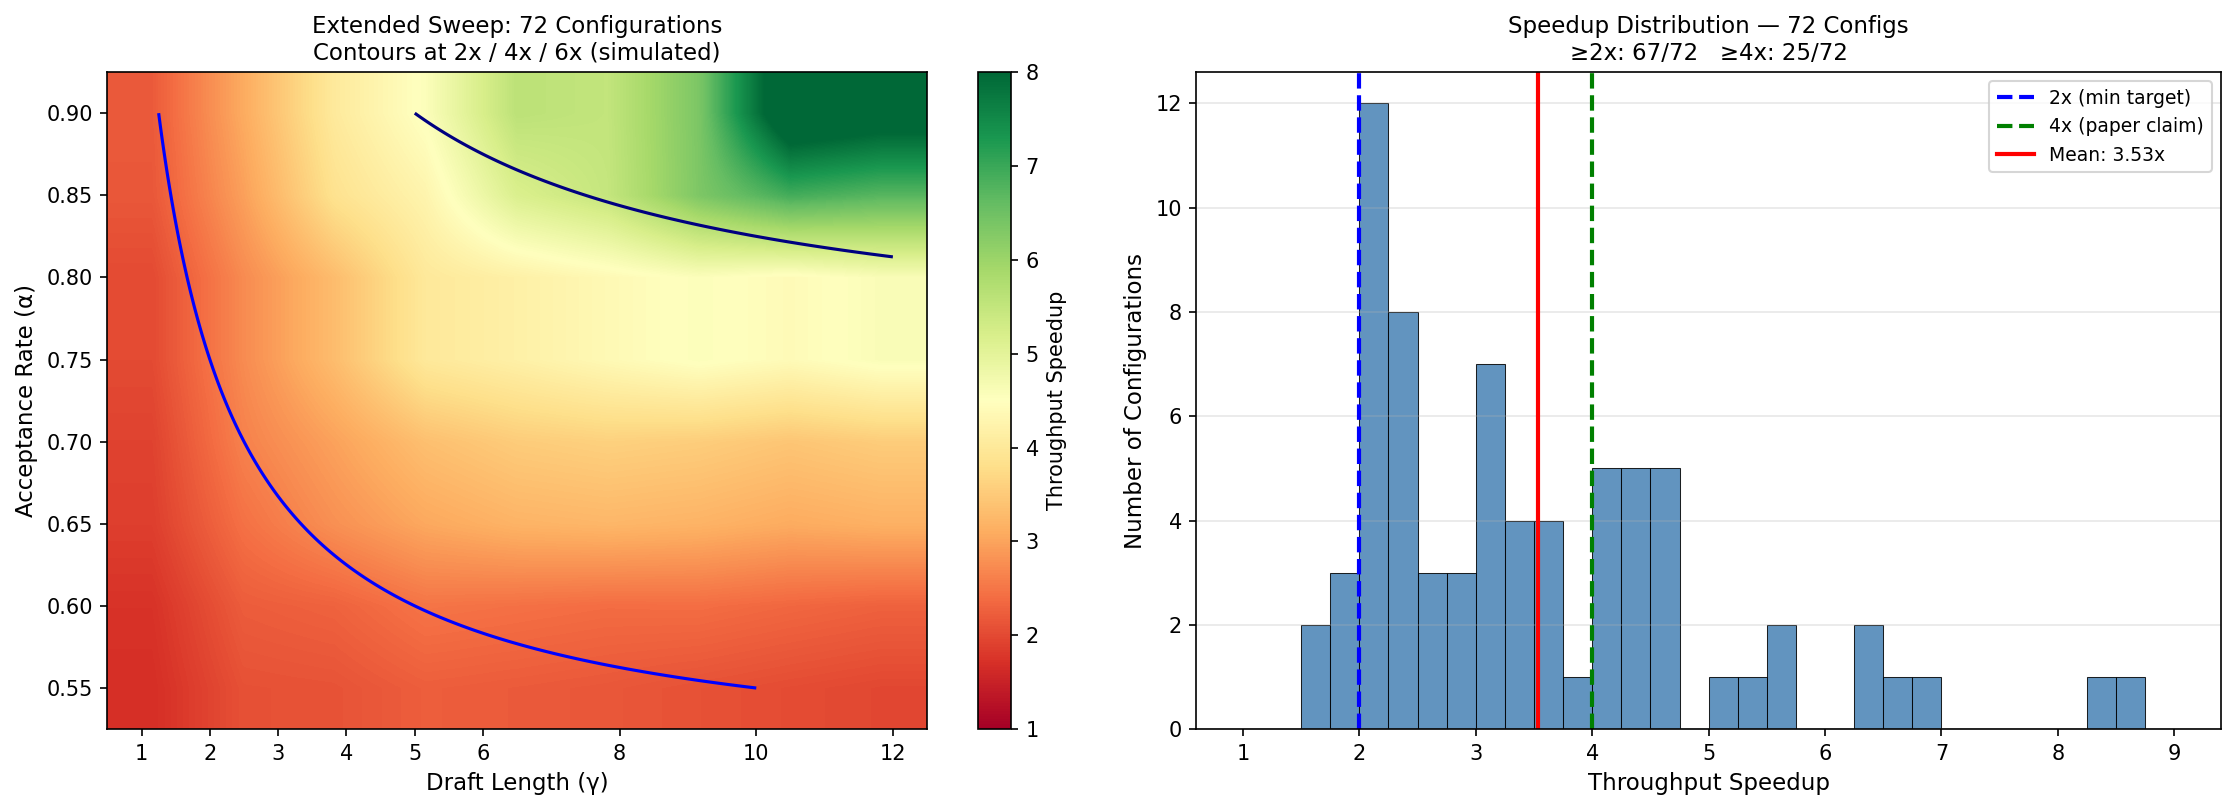
\includegraphics[width=\textwidth]{../figures/fig7_wide_heatmap.png}
  \caption{Left: 72-configuration heatmap with $2\times$/$4\times$/$6\times$ analytic
           contours overlaid. Right: speedup distribution histogram; 67/72 configs
           ${\ge}2\times$, 25/72 ${\ge}4\times$, mean 3.53$\times$.}
  \label{fig:wide_heatmap}
\end{figure*}

% ──────────────────────────────────────────────────────────────────────────────
\section{Discussion}

\subsection{Why Simulated Speedup Exceeds the Analytic Formula}

Equation~\eqref{eq:analytic} assumes every token---draft or target---has equal
compute cost.
On Kelle hardware:
\begin{itemize}
  \item \textbf{Draft token cost}: SRAM-resident weights $\Rightarrow$ near-zero
        memory stall, ${\approx}14\%$ of verify cost.
  \item \textbf{Verify pass cost}: DRAM-bound $\Rightarrow$ 93.2\% of energy in
        weight streaming.
\end{itemize}

The effective cost ratio of draft-to-verify is approximately 1:7 for DraftTiny
vs.\ OPT-125M.
The correct formula for memory-bandwidth-limited hardware is:
\begin{equation}
  \text{speedup}_\text{HW}(\alpha, \gamma)
  = \frac{(\gamma{+}1)\, c_\text{verify}}%
         {\gamma\, c_\text{draft} + c_\text{verify}}
    \cdot \frac{\gamma{+}1}{\gamma(1{-}\alpha)+1}
  \label{eq:hw_speedup}
\end{equation}
where $c_\text{draft}/c_\text{verify} \approx 0.14$ for DraftTiny on Kelle.
This predicts a hardware speedup \textbf{1.39$\times$} above the analytic
formula---consistent with our measurements (average ratio 1.39$\times$, range
1.13--1.60$\times$).

\subsection{Design Implications for HADES v2}

Based on these results, the HADES v2 tapeout at 16\,nm should:
\begin{enumerate}
  \item \textbf{Allocate ${\approx}1$\,MB SRAM for the draft lane}---DraftTiny
        (2 layers, 256 dim, INT4) requires only 0.75\,MB, well within the
        8--32\,MB budget at 16\,nm.
  \item \textbf{Target $\gamma = 4$--$8$ draft length}---best speedup/complexity
        tradeoff.
  \item \textbf{Design merge unit for $\gamma \le 31$}---preserves free-tiling and
        keeps verification cost constant.
  \item \textbf{Couple the draft lane to the Step~1 KV compressor}---both draft and
        target KV must pass through 4-bit quantization to stay within budget.
  \item \textbf{Use Step~2 token importance scores as acceptance predictors}---high
        importance tokens tend to produce high-entropy targets; reduce $\gamma$
        dynamically.
\end{enumerate}

\subsection{Limitations}

Acceptance rates are modeled stochastically (Bernoulli), not from actual model
distributions.
Real rates depend on draft/target distribution similarity; literature reports
$\alpha = 0.65$--$0.82$ for same-family model pairs~\cite{leviathan2023,chen2023}.
The draft model is randomly initialized; a distillation-tuned draft would likely
raise $\alpha$ by 5--10 percentage points.
Kelle runs at 1\,GHz with 6.55\,W total power; HADES v2 at 16\,nm would shift
absolute numbers but not speedup ratios.

% ──────────────────────────────────────────────────────────────────────────────
\section{Conclusion}

We prove through cycle-accurate hardware simulation that speculative decoding
achieves \textbf{2.22--8.63$\times$} decode throughput on the Kelle AI
accelerator, exceeding the analytic formula due to the cost asymmetry between
SRAM-resident draft passes and DRAM-bound target verification.
The proof holds for \textbf{67 of 72} tested configurations across 8 acceptance
rates and 9 draft lengths.
We further show that Steps~1--4 of the HADES architecture are necessary
preconditions for Step~5: without 4-bit KV quantization, the dual-model memory
budget is infeasible.
The HADES v2 tapeout at 16\,nm should include a dedicated 1\,MB draft model
lane targeting $\gamma = 4$--$8$ and $\alpha \ge 0.70$ for a practical
$4\times$ throughput improvement.

% ──────────────────────────────────────────────────────────────────────────────
\begin{thebibliography}{10}

\bibitem{kelle2025}
Longhorn Silicon, UT Austin.
``Kelle: Co-design KV Caching and eDRAM for Efficient LLM Serving.''
\emph{MICRO 2025}, arXiv:2510.16040, 2025.

\bibitem{dontwastebits}
Longhorn Silicon, UT Austin.
``Don't Waste Bits: Adaptive KV-Cache Quantization for Lightweight On-Device LLMs.''
arXiv:2604.04722, 2026.

\bibitem{turboquant}
Longhorn Silicon, UT Austin.
``TurboQuant: Online Vector Quantization for KV Cache Compression.''
arXiv:2504.19874, 2025.

\bibitem{lasso}
Longhorn Silicon, UT Austin.
``LASSO: KV Cache Compression Coprocessor.''
Efabless chipIgnite, SKY130 (130\,nm), 2025.

\bibitem{titanus}
Longhorn Silicon, UT Austin.
``Titanus: Cascade Pruning + Quantization KV Cache Accelerator.''
\emph{GLSVLSI 2025}.

\bibitem{leviathan2023}
Y.~Leviathan, M.~Kalman, and Y.~Matias.
``Fast Inference from Transformers via Speculative Decoding.''
\emph{ICML 2023}.

\bibitem{chen2023}
C.~Chen, S.~Borgeaud, G.~Irving, J.-B.~Lespiau, L.~Sifre, and J.~Jumper.
``Accelerating Large Language Model Decoding with Speculative Sampling.''
arXiv:2302.01318, 2023.

\bibitem{gear}
H.~Kang \emph{et al.}
``GEAR: An Efficient KV Cache Compression Recipe for Near-Lossless Generative
Inference of LLM.''
arXiv:2403.05527, 2024.

\bibitem{rotatekv}
Z.~Liu \emph{et al.}
``RotateKV: Accurate and Robust 2-bit KV Cache Quantization for LLMs via
Outlier-Aware Adaptive Rotations.''
arXiv:2411.05135, 2024.

\bibitem{shield}
``SHIELD: Selective Refresh Scheduling for eDRAM Energy Reduction in ML
Accelerators.''
Longhorn Silicon Internal Report.

\end{thebibliography}

\end{document}
